\documentclass{article}
\usepackage[utf8]{inputenc}
\usepackage[english]{babel}
\usepackage[]{amsthm} %lets us use \begin{proof}
\usepackage[]{amssymb} %gives us the character \varnothing
\usepackage[]{setspace} %provides commands to set line spacing
\usepackage[left=0.75in, right=0.75in]{geometry}
\usepackage{hyperref}
\usepackage{xcolor}
\usepackage{graphicx}
\usepackage{caption}
\usepackage{subcaption} % For subfigures
\usepackage{float} % For the H float option
%\author{Son Nguyen}
%\date{\today}

\begin{document}
%\maketitle %This command prints the title based on information entered above
\begin{center}
    \LARGE{Machine Learning for VQE}\\[1em]
    \large Son Nguyen\\[1em]
    %\large \today
\end{center}

\onehalfspacing

%%%%%%%%%%%%%%%%%%%%%%%%%%%%%%%%%%%%%%%%%%%%%%%%%%%%%% Content %%%%%%%%%%%%%%%%%%%%%%%%%%%%%%%%%%%%%%%%%%%%%%%%%%%%%%%%%%%%%%%%%%%%%%%%%%%%%%%%5

\subsection*{Optimizing parameters}

We have a quantum state \(|\psi(\vec{\theta})\rangle\), where \(\vec{\theta} = (\theta_1, \theta_2, \theta_3, \dots, \theta_n)\) are the parameters of the quantum circuit. The goal is to find the optimal \(\theta\) that minimizes the expectation value of the Hamiltonian \(H\). \\
\\
The cost function to minimize the expectation value (energy) of the Hamiltonian is given by:

\[E (\vec{\theta}) = \langle \psi(\vec{\theta})|H|\psi(\vec{\theta})\rangle\]

\noindent The optimizer's goal is to find the set of parameters \(\vec{\theta}\) that \(E(\vec{\theta})\).

\subsection*{Gradient-based optimization}

Gradient descent is a common type of optimizer. It uses the gradient of the cost function with respect to the parameters:

\[\theta^{(t+1)}_i = \theta^{(t)}_i - \eta \nabla E(\vec{\theta}^{(t)})\]

\noindent Where:
\begin{itemize}
    \item \(\eta\) is the learning rate.
    \item \(\theta^{(t)}_i\) is the parameter at iteration t.
    \item \(\nabla E(\vec{\theta}^{(t)})\) is the gradient of the cost function with respect to the parameter \(\theta_i\).
\end{itemize}
The optimizer will stop when \(|E(\vec{\theta}^{(t+1)})- E(\vec{\theta}^{(t)})| \) is smaller than threshold \(\epsilon\).

The final parameters \(\vec{\theta}^*\) will be those that minimzie the energy. The ansatz state \(|\psi(\vec{\theta^*})\rangle\) approximates the ground state of the Hamiltonian.

Parameter-Shifting Rule for parameter \(\theta_i\):
\[\nabla E(\vec{\theta}^{(t)}) = \left(\frac{\partial E(\vec{\theta})}{\partial\theta_0},\frac{\partial E(\vec{\theta})}{\partial\theta_1},\frac{\partial E(\vec{\theta})}{\partial\theta_2},\dots,\frac{\partial E(\vec{\theta})}{\partial\theta_n}\right)\]
\[\frac{\partial E(\vec{\theta})}{\partial\theta_i} \approx \frac{E\left(\vec{\theta} + s_k\right) - E\left(\vec{\theta} - s_k\right)}{2s_k}\]

where \(s_k\) is a  unit shift in the k-th parameter, i.e., \(s_k\) = (0, . . . , 0, sk, 0, . . . , 0) with  \(s_k \neq 0\). The parameter-shift rule allows us to estimate the gradient using the difference between the cost function evaluated at two nearby points in parameter space.


The gradient-based algorithm rely on direct measurement of the gradient of the loss function with respect to the parameters being optimized. These measurement 
typically yeild an estimate of the gradient because the underlying data usually include added noise which is inherent to the quantum system.
\subsection*{SPSA - simultaneous perturbation stochastic approximation}

SPSA is a gradient-free optimization method that 
estimates the gradient using a finite difference method. 
It is robust to noise and does not require the gradient to be calculated analytically. While executing a variational algorithm using a Quantum Assembly Language (QASM)
simulator or a real device, SPSA would be the most recommended choice among the optimizers.

    \begin{enumerate}
    \item Initialize the parameters \(\vec{\theta}\).
    \item For each iteration:
    \begin{enumerate}
        \item Randomly choose a perturbation vector \(\vec{\Delta}\) with elements \(\pm 1\) (Bernoulli distribution with probability of \(\frac{1}{2}\) for each \(\pm 1\) outcome).
        \item Perturbation Step. Let \(\vec{\theta}^{(t)}\) be the parameter vector at iteration t. The pertubed parameter vectors are:
        \[\vec{\theta}^{(t)}_+ = \vec{\theta}^{(t)} + c^{(t)} \Delta\vec{\theta}^{(t)}\]
        \[\vec{\theta}^{(t)}_- = \vec{\theta}^{(t)} - c^{(t)} \Delta\vec{\theta}^{(t)}\]
        where \(c^{(t)}\) is is a small perturbation factor that decreases over iterations. 
        \item The quantum circuit is executed twice for each iteration, once with \(\vec{\theta}^{(t)}_+\) and once with \(\vec{\theta}^{(t)}_-\). The expectation value of the Hamiltonian is measured for each circuit execution.
        \[E(\vec{\theta}^{(t)}_+)= \langle \psi(\vec{\theta}^{(t)}_+)|H|\psi(\vec{\theta}^{(t)}_+)\rangle\]
        \[E(\vec{\theta}^{(t)}_-)= \langle \psi(\vec{\theta}^{(t)}_-)|H|\psi(\vec{\theta}^{(t)}_-)\rangle\]
        \item Gradient approximation. SPSA approximates the gradient for each parameter based on the difference in energy between the 2 perturbed states:
        \[\hat{g}^{(t)}_i = \frac{E(\vec{\theta}^{(t)}_+) - E(\vec{\theta}^{(t)}_-)}{2c^{(t)}\Delta\theta^{(t)}_i}\]
        The entire gradient vector \(\hat{g}^{(t)}\) is computed with just 2 evaluations of the cost function, regardless of the number of parameters. 
        \item Update the parameters:
        \[\vec{\theta}^{(t+1)} = \vec{\theta}^{(t)}-a^{(t)}\hat{g}^{(t)}\]
        where \(a^{(t)}\) is the learning rate that decreases over iterations.\\
        Parmaters Schedule:        
        \[a^{(t)} = \frac{a}{(A + t + 1)^\alpha}\]
        \[c^{(t)} = \frac{c}{(t+1)^\gamma}\]
        where A, \(\alpha\), \(\gamma\) control the decay of the learning rate and perturbation factor.
    \end{enumerate} 
    \end{enumerate}

    \begin{figure}[H]
        \centering
        \begin{subfigure}[b]{0.45\textwidth}
            \centering
            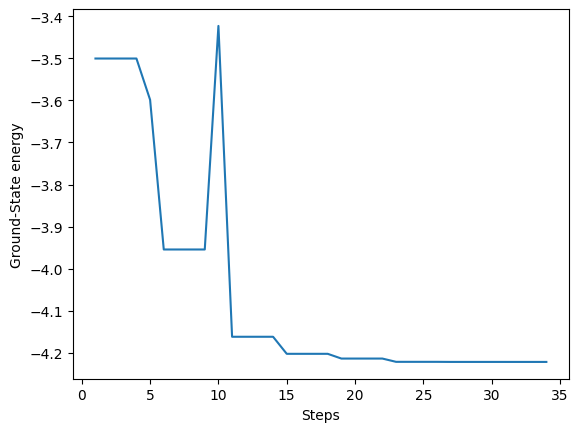
\includegraphics[width=\textwidth]{Pasted image 1.png}
            \caption{Optimizing the Cost Function (Energy)}
        \end{subfigure}
        \hfill
        \begin{subfigure}[b]{0.45\textwidth}
            \centering
            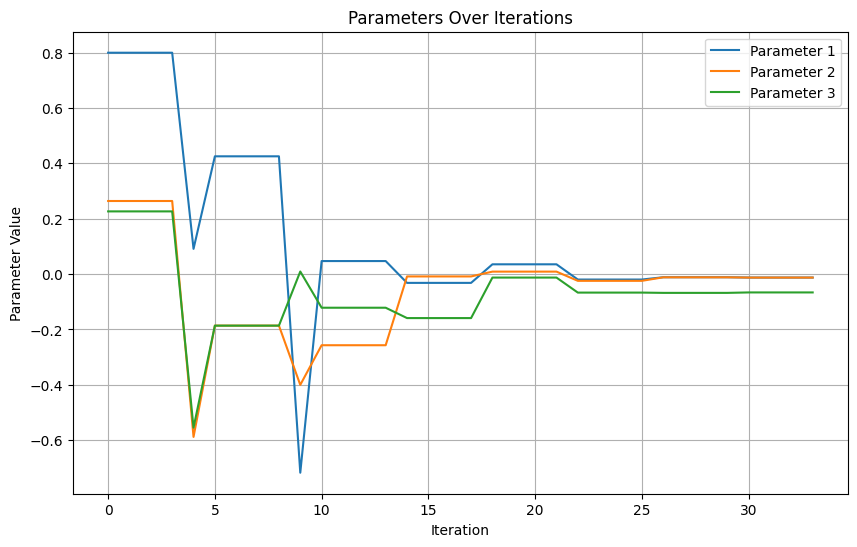
\includegraphics[width=\textwidth]{Pasted image.png}
            \caption{Parmaters change over iterations}
        \end{subfigure}
        \caption{The optimization process using SPSA method (HeH+ molecule)}
    
    
    \end{figure}
\subsection*{References}
\begin{itemize}
    \item \href{https://www.jhuapl.edu/SPSA/PDF-SPSA/Spall_An_Overview.PDF}{Simultaneous Perturbation Stochastic Approximation}
    \item \href{https://physlab.org/wp-content/uploads/2023/05/Quantum_Gradient_Descent_24100266_Fin.pdf#:~:text=The%20parameter%20shift%20rule%20is%20a%20crucial%20technique,parameter%20%CE%B8i%20can%20be%20computed%20as%3A%20%E2%88%82%E2%9F%A8O%E2%9F%A9%201}{Quantum Gradient Descent}
\end{itemize}
\end{document}